% Extended explanatory companion to the JAES Engineering Report.
\documentclass[11pt,a4paper]{article}

\usepackage{amsmath,amssymb}
\usepackage{graphicx,booktabs,array}
\usepackage[top=3cm,bottom=4cm,left=25mm,right=25mm]{geometry}
\usepackage[square,comma,numbers,sort&compress]{natbib}
\usepackage[T1]{fontenc}
\usepackage{mathtools}
\usepackage{newpxtext}
\usepackage{newpxmath}
\usepackage{fancyhdr}
\usepackage{lastpage}
\usepackage[mathlines]{lineno}
\usepackage{siunitx}
\usepackage{xurl}

% Metadata loads hyperref.
% Auto-generated DO NOT EDIT
    \usepackage[
        pdfauthor={Luc Holtkamp},
        pdftitle={Datasheet-Based Ranking of Sealed-Box Bass Drivers for a Small-Area DSP-Integrated Stereo System v3.0},
        pdfsubject={A Parameterized Datasheet-Based Screening and Architecture-Comparison Procedure for a Small-Area DSP-Integrated Stereo Bass System},
        pdfkeywords={['loudspeaker driver selection', 'sealed enclosure', 'Pareto ranking', 'stereo bass', 'room gain', 'nonlinear headroom']},
    ]{hyperref}
    
    \newcommand{\PaperTitle}{Datasheet-Based Ranking of Sealed-Box Bass Drivers for a Small-Area DSP-Integrated Stereo System}
    \newcommand{\PaperVersion}{v3.0}
    \newcommand{\PaperAuthor}{Luc Holtkamp}
    \newcommand{\PaperSummary}{A Parameterized Datasheet-Based Screening and Architecture-Comparison Procedure for a Small-Area DSP-Integrated Stereo Bass System}
    \newcommand{\PaperCopyright}{Luc Holtkamp (SenseMagic), 2013--2026}
    \newcommand{\PaperLicense}{CC BY 4.0}
    \newcommand{\PaperEmail}{luc@sensemagic.nl}
    \newcommand{\PaperWebsite}{www.sensemagic.nl}
    \newcommand{\PaperAfiliation}{SenseMagic, Netherlands}
    
\usepackage[capitalise]{cleveref}

% Build toggle: 0 = branded explanatory preprint (default), 1 = plain
% journal-style companion.  A driver file may define \ELSVIERBUILD before
% inputting this file.
\providecommand{\ELSVIERBUILD}{0}

\parindent 0pt
\parskip 1ex
\setlength{\headheight}{40pt}
\setlength{\footskip}{40pt}
\renewcommand{\baselinestretch}{1.33}
\numberwithin{equation}{section}
\renewcommand{\bibname}{References}
\renewcommand{\contentsname}{Contents}
\bibliographystyle{unsrtnat}

% refs.bib contains a month expression that produces these commands.
\providecommand{\slash}{/}
\providecommand{\slashFeb}{/Feb}
\providecommand{\slashFebruary}{/February}

\newcommand{\Sd}{S_{\mathrm{d}}}
\newcommand{\Xmax}{X_{\mathrm{max}}}
\newcommand{\Vd}{V_{\mathrm{d}}}
\newcommand{\Mms}{M}
\renewcommand{\Re}{R_{\mathrm{e}}}
\newcommand{\Le}{L_{\mathrm{e}}}
\newcommand{\Rms}{R_{\mathrm{m}}}
\newcommand{\Cms}{C_{\mathrm{m}}}
\newcommand{\Bl}{Bl}
\newcommand{\Qes}{Q_{\mathrm{es}}}
\newcommand{\Qms}{Q_{\mathrm{ms}}}
\newcommand{\Qts}{Q_{\mathrm{ts}}}
\newcommand{\Qtc}{Q_{\mathrm{tc}}}
\newcommand{\Qmc}{Q_{\mathrm{mc}}}
\newcommand{\Vas}{V_{\mathrm{as}}}
\newcommand{\Vb}{V_{\mathrm{b}}}
\newcommand{\Pmax}{P_{\mathrm{max}}}
\newcommand{\ws}{\omega_{\mathrm{s}}}
\newcommand{\wc}{\omega_{\mathrm{c}}}
\newcommand{\se}{\sigma_{\mathrm{e}}}
\newcommand{\sm}{\sigma_{\mathrm{m}}}
\newcommand{\dd}{\mathrm{d}}

\begin{document}

\ifnum\ELSVIERBUILD=1
	% Plain journal-submission title page: title, author, affiliation,
% corresponding author -- no cover art, no copyright/license/version branding
% (those belong to the preprint only; a journal captures license/affiliation
% via its submission system, and typesets its own running headers/footers).
% Used when \ELSVIERBUILD = 1.
%=============================================================================================================================
\begin{titlepage}
%=============================================================================================================================
\thispagestyle{empty}

\begin{center}

	{\Huge \PaperTitle \par}

	\vspace{1.5em}

	{\large \PaperAuthor$^{a,\ast}$ \par}

	\vspace{0.5em}

	{\normalsize $^{a}$\PaperAfiliation \par}

	\vspace{2em}

	{\normalsize
		$^\ast$Corresponding author. \\
		\textit{Email address:} \texttt{\PaperEmail} (\PaperAuthor)
		\par}

\end{center}

%=============================================================================================================================
\end{titlepage}
%=============================================================================================================================

\else
	% Branded preprint title page (SenseMagic identity).
% Used when \ELSVIERBUILD = 0 (the default / preprint build).
%=============================================================================================================================
\begin{titlepage}
%=============================================================================================================================

%Make our own title on an empty page (without footer and header)
%See fancyhdr.pdf
\fancypagestyle{empty}
\lhead{}
\chead{}
\rhead{}
\lfoot{}
\lfoot{}
\cfoot{}
\rfoot{}
\renewcommand{\headrulewidth}{0pt}
\renewcommand{\footrulewidth}{0pt}

\begin{center}
	
	{\Huge \PaperTitle \par}
	
	\vspace{1em}
	
	{\Large \PaperSummary \par}
	
	\vspace{1.5em}
	
	{\large \PaperAuthor \par}
	{\normalsize \PaperAfiliation \par}
	{\normalsize \texttt{\PaperEmail} \par}
	
	\vspace{5cm}
	
\end{center}

%=============================================================================================================================
\end{titlepage}
%=============================================================================================================================

\fi

\linenumbers

\section*{Abstract}

This document is the extended explanatory companion to the stabilized JAES
Engineering Report.  It presents a reproducible pre-purchase procedure for
screening and ranking sealed-box bass drivers for one declared system: a
compact prepared living-room couch area, half-space soffit mounting, a shared
mono low-bass manifold, independent stereo upper-bass channels, and
finite-band DSP alignment.  Classical sealed-box relations are derived in
detail and placed on explicit reference bases.  Feasibility is checked across
each complete role band against excursion, enclosure volume, voice-coil
dissipation, amplifier voltage, amplifier current, continuous power, burst
power, and a rough inductive screen.  Low-frequency demand is obtained from a
leaky pressure-zone limiting model and tested for sensitivity to room leakage.
Transient demand is obtained by numerical integration of the sealed ODE for a
declared one-cycle waveform family, including ring-down.  Excursion, Doppler
sideband ratio, box-spring asymmetry, electrical utilization, and inductive
uncertainty remain separately reported indicators.  Surviving candidates
receive role-specific Pareto fronts and lexicographic orders.  Aggregate
evidence comes from a hash-identified private database without redistributing
its rows; the worked system uses public manufacturer records.  The result is
an application-specific shortlist, not a new physical limit or a claim about
all loudspeaker architectures.

\vspace{1em}
\noindent\textbf{Keywords:} loudspeaker driver selection; sealed enclosure;\\
maximum acoustic output; datasheet screening; room gain; nonlinear headroom

\ifnum\ELSVIERBUILD=1
	% Plain running header/footer for a journal submission build: page numbers
% only, no branding, license, or version string (most journals typeset their
% own running heads in production; the license/version are not relevant to
% the review copy). Used when \ELSVIERBUILD = 1.
\pagestyle{plain}

\else
	% Branded running header/footer for the preprint build (copyright, license,
% version, filename). Used when \ELSVIERBUILD = 0 (the default / preprint
% build).
\pagestyle{fancy}
\lhead{}
\chead{}
\rhead{\large \PaperTitle \vspace{1mm}}
\lfoot{\parbox[t]{0.6\textwidth}{ \footnotesize
        \textcopyright\ \PaperCopyright \\
        Licensed under \PaperLicense  \\
        Contact: \texttt{\PaperEmail} \textbullet\ \texttt{\PaperWebsite} }}
\cfoot{}
\rfoot{\parbox[t]{0.34\textwidth} {\footnotesize
		\hfill 
    \begin{tabular}[t]{l l}
        Page:    & \thepage\ of \pageref{LastPage} \\
        File:    &  \jobname \\
        Version: & \PaperVersion
    \end{tabular} }}
\renewcommand{\headrulewidth}{0.5pt}
\renewcommand{\footrulewidth}{0.5pt}

\fi

\tableofcontents
\clearpage

\section{Purpose, status, and system architecture}
\label{sec:intro}

\subsection{Status of this document}

This is a detailed explanatory companion, not the submitted JAES manuscript.
The condensed Engineering Report is the publication document; this companion
retains intermediate algebra, implementation details, and additional
interpretation that would be too long for the journal format.  Both documents
use the same canonical scenario, generated figures, generated tables,
public-driver records, and ranking policy.  The equations below distinguish
three kinds of statements:

\begin{itemize}
	\item established small-signal loudspeaker and room relations that are
	rederived to fix notation and conventions;
	\item exact consequences of the stated lumped model;
	\item declared engineering choices, empirical observations, and risk
	indicators whose scope is narrower than the equations.
\end{itemize}

The method is intended for the stage before drivers are purchased, when the
available evidence is principally public Thiele/Small fields and manufacturer
ratings.  It narrows a population to defensible candidates.  It does not
replace impedance, near-field, large-signal, thermal, or in-room measurement
of the purchased units.

\subsection{Fixed application}
\label{sec:intro-arch}

\Cref{fig:architecture} fixes the system to which every result applies:

\begin{itemize}
	\item a compact primary listening area centred on a prepared living-room
	couch and represented by a declared reference response or an aggregate
	over a small declared measurement set;
	\item half-space soffit-wall mounting for the bass sources;
	\item a common mono low-bass manifold covering
	\SIrange{15}{80}{\hertz};
	\item independent left and right upper-bass channels covering
	\SIrange{80}{250}{\hertz};
	\item finite-band crossover, magnitude correction, phase alignment, and
	delay alignment;
	\item one amplifier channel per physical driver.
\end{itemize}

The low-bass target is \SI{110}{dB} for the complete four-driver manifold.
Its drivers share one signal, so each supplies one quarter of the required
peak displaced volume.  The upper-bass target is \SI{105}{dB} for each
stereo channel independently.  The opposite channel contributes no sizing
credit because ordinary stereo programme is not guaranteed to be correlated.
Electrical demand is always calculated for each physical driver.

\begin{figure}[htbp]
	\centering
	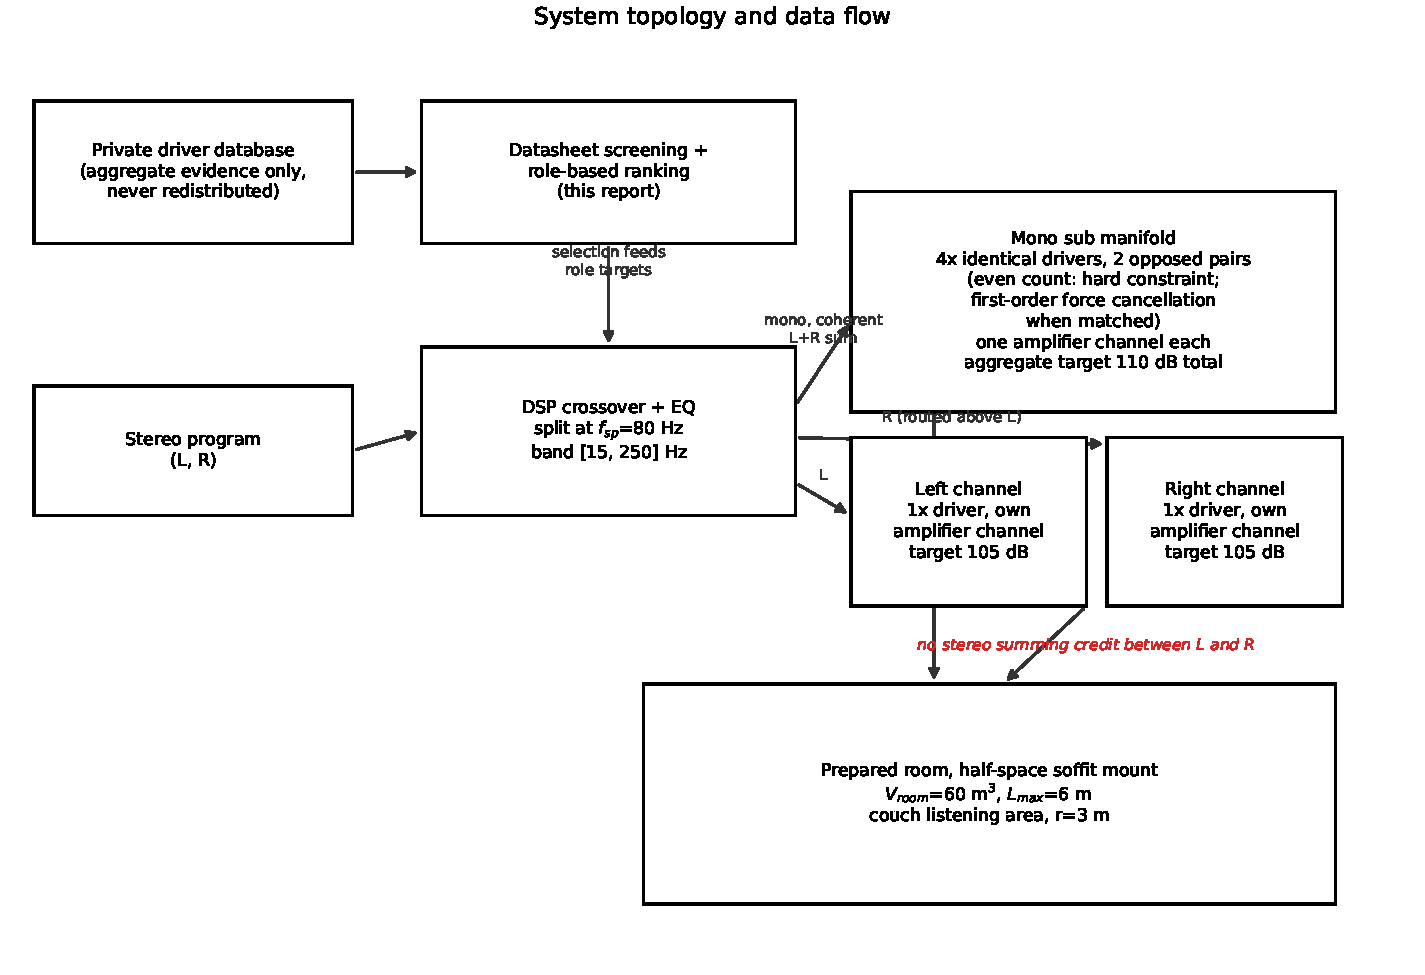
\includegraphics[width=0.92\textwidth]{figures/fig_architecture}
	\caption{Canonical architecture and data flow.  The procedure accepts
	public datasheet fields, a declared room and couch-area basis, separate
	role targets, enclosure constraints, amplifier limits, and a transient
	test specification.  It returns separate low-bass and upper-bass orders;
	the role indicators are not collapsed into one cross-role score.}
	\label{fig:architecture}
\end{figure}

\subsection{Scene fidelity and its boundary}
\label{sec:intro-fidelity}

The architectural aim is high fidelity to the recorded two-channel scene
over the primary couch area: stable localization and image focus, accurate
direct- and early-field timbre, controlled low-frequency summation, and
coherent integration across the crossover.  In a small room these attributes
depend on the direct sound and early reflections \cite{toole2006,bech1998},
on the relative phase and delay of noncoincident sources
\cite{linkwitz1976}, and on group-delay error \cite{blauert1978}.  Soffit
mounting, room preparation, compact source geometry, and finite-band DSP make
those variables more controllable over a small area than an objective based
only on diffuse-field level.

That rationale is not a listening-test result.  It also concerns scene
fidelity rather than listener envelopment.  Envelopment depends strongly on
late lateral energy \cite{bradley1995,rumsey2002} and may be better served by
multichannel or deliberately diffuse reproduction \cite{francombe2017}.
Likewise, multi-seat low-frequency uniformity is a different optimization
problem \cite{welti2006}.  The present architecture accepts reduced off-area
robustness in exchange for tighter control of one prepared couch area.

\subsection{Contribution}
\label{sec:intro-contribution}

No new motor law or enclosure physics is claimed.  The contribution is the
integration of established relations into a complete decision path:

\begin{enumerate}
	\item normalize public records and preserve uncertainty about rating
	conventions;
	\item choose a realizable sealed alignment under a finite box cap;
	\item convert a declared couch-area target and room transfer into required
	displaced volume over each complete role band;
	\item compute steady and finite-burst displacement, voltage, current, and
	coil dissipation per driver;
	\item reject any record that crosses a hard gate;
	\item report separate nonlinear-risk and implementation indicators;
	\item construct role-specific Pareto fronts and then apply a declared
	lexicographic order;
	\item test whether the resulting shortlist is stable under plausible
	datasheet, room, and policy perturbations.
\end{enumerate}

\section{Previous work and positioning}
\label{sec:prevwork}

\begin{table*}[htbp]
\centering
\caption{Established prior results integrated by this report vs. its own methodological and policy contribution.}
\label{tab:prior-art}
\begin{tabular}{p{5.1cm}p{2.6cm}p{6.7cm}}
\toprule
element & class & this report's treatment\\
\midrule
Sealed-box alignment, Thiele/Small closed-box theory & established prior result & reused unchanged as the sealed-box ODE and alignment line\\
Displacement-limited output ceiling ($V_d=S_dX_{\max}$) & established prior result & used as an exact descriptor, not a universal loudspeaker optimum\\
Thermal (dissipation-limited) output ceiling ($\eta_0P_{\max}$) & established prior result & used as an exact descriptor; never summed with the displacement ceiling\\
$X_{\max}$ as an IEC/Klippel excursion anchor & established prior result & used only as the clipping boundary; not converted into absolute THD\\
Room pressure-zone compliance below the first mode & established prior result & extended with an explicit first-order leakage-corner term; used only as a first-pass sizing/limiting model, not a claim about the complete room\\
Doppler (FM) sideband index & established prior result & reported as a separate, non-summed nonlinear-risk indicator\\
Finite-band DSP room correction & established prior result & adopted as an explicit scope input rather than an unconstrained assumption\\
Role-specific, non-compensatory ranking policy (mono sub manifold vs. independent stereo upper-bass channels) & this report's contribution & declared engineering policy; separate Pareto fronts per role, no cross-role or cross-channel summing credit\\
Explicit finite-amplifier feasibility gates (voltage, current, continuous and burst power) & this report's contribution & integrated into every role evaluation and the worked example\\
Numerical sealed-ODE transient (burst) displacement factor & this report's contribution & replaces a constant free-mass burst factor near $F_c$\\
Aggregate, hash-verified private-database screening evidence & this report's contribution & counts and hexbin/histogram population evidence only, no row-level redistribution\\
\bottomrule
\end{tabular}
\end{table*}


Closed-box synthesis, alignment, reference efficiency, and maximum-output
relations follow Small \cite{small1972,small1972direct}.  Fielder and
Benjamin \cite{fielder1988} connect subwoofer displacement to programme and
room requirements and are the nearest precedent for the sizing side of this
work.  The present contribution is not a replacement for either body of
work; it is a reproducible policy layer that carries those relations through
to a finite enclosure, finite electronics, a declared room, and a candidate
order.

The efficiency-bandwidth product
\begin{equation}
	EBP=\frac{F_s}{\Qes}
	\label{eq:ebp}
\end{equation}
is widely used as a first enclosure-type screen \cite{dickason2006}.  It is
related to electrical damping and therefore contains useful motor-to-mass
information.  It does not state target distance, room transfer, box volume,
available stroke, rated dissipation, or amplifier headroom.  This procedure
uses the exact corner rate $F_s/\Qts$ for alignment and never uses $EBP$ as a
standalone performance order.

Published $\Xmax$ values may be geometric, distortion-defined, or based on a
manufacturer-specific rule \cite{iec62458,klippel2003xmax,klippel2006}.
Power ratings likewise depend on test standard and duration \cite{aes2}.
The procedure therefore records the source and basis when available and
perturbs both fields during robustness analysis.

Large-signal motor and suspension behaviour is described by parameters such
as $Bl(x)$, $K_{\mathrm{ms}}(x)$, and $L_{\mathrm e}(x,i)$
\cite{klippel2006}.  Datasheet fields do not provide those curves.  The
indicators used here consequently express proximity to declared boundaries,
not a predicted acoustic percentage.  Doppler frequency modulation has a
long literature and a disputed audibility interpretation
\cite{klipsch1969,allison1982}; only the kinematic first-sideband ratio is
used.  Thermal compression requires resistances and time constants that are
not recoverable from a continuous-power number alone \cite{button1992}.

Room response is spatially distributed.  Toole \cite{toole2006} describes
the distinction between direct/early-field behaviour and the modal region;
Welti and Devantier \cite{welti2006} optimize low-frequency response over a
defined seating region; modal equalization and multi-position correction are
bounded by measurement geometry and regularization
\cite{makivirta2003,cecchi2018}.  Those results motivate the explicit
couch-area reference and the refusal to treat DSP as exact inversion.

Finally, vented loading is established fourth-order practice
\cite{small1973vented}.  Port compression and turbulence are design
constraints with known mitigations \cite{salvatti2002,vanderkooy1998}.
\Cref{sec:vented} therefore compares sealed and vented loading only under
the present system constraints.

\section{Scope, conventions, and canonical scenario}
\label{sec:scope}

\subsection{Notation and reference bases}
\label{sec:scope-bases}

SI units are used.  Unless otherwise stated,
$\rho_0=\SI{1.20}{\kilogram\per\cubic\meter}$,
$c=\SI{343}{\meter\per\second}$, and $p_0=\SI{20}{\micro\pascal}$.
Sound pressure levels use rms pressure.  Cone displacement, displaced
volume, and sinusoidal phasor amplitudes marked with a hat are peak values.
Voltage and current limits are rms values; power is mean coil dissipation
over the stated interval.

\begin{center}
\small
\begin{tabular}{@{}llll@{}}
\toprule
$F_s$ & free-air resonance & $\Mms$ & moving mass\\
$\Qes,\Qms,\Qts$ & quality factors & $\Re$ & dc resistance\\
$\Vas$ & compliance volume & $\Bl$ & force factor\\
$\Sd$ & effective piston area & $\Le$ & voice-coil inductance\\
$\Xmax$ & one-way excursion boundary & $\Pmax$ & rated dissipation\\
$\Vd$ & $\Sd\Xmax$ & $\Vb$ & net sealed-box volume\\
$F_c,\Qtc$ & in-box resonance and Q & $f_L$ & inductive screen\\
\bottomrule
\end{tabular}
\end{center}

Four pressure bases must remain distinct:

\begin{enumerate}
	\item[B1.] \textbf{Intrinsic ceiling}: one driver, half space,
	$r=\SI{1}{\meter}$.  This characterizes a driver only.
	\item[B2.] \textbf{Couch-area demand}: required pressure at the declared
	listening distance and response aggregation.
	\item[B3.] \textbf{Mono-manifold total}: aggregate low-bass pressure at
	B2.  The common displaced-volume demand is divided among the manifold
	drivers.
	\item[B4.] \textbf{One stereo channel}: the pressure required from one
	upper-bass channel at B2.
\end{enumerate}

\subsection{Canonical numerical scenario}
\label{sec:scope-scenario}

\begin{center}
\small
\begin{tabular}{@{}p{4.0cm}p{9.4cm}@{}}
\toprule
room & $V_{\mathrm{room}}=\SI{60}{\cubic\meter}$,
$L_{\max}=\SI{6}{\meter}$; prepared for the stated source/listening area\\
couch-area distance & $r_{\mathrm{listen}}=\SI{3}{\meter}$\\
room limiting model & leaky pressure zone, $f_\ell=\SI{10}{\hertz}$\\
role bands & mono low bass \SIrange{15}{80}{\hertz};
upper bass \SIrange{80}{250}{\hertz}\\
targets & \SI{110}{dB} complete mono manifold;
\SI{105}{dB} independently per stereo channel\\
mounting and correction & half space; finite-band DSP\\
alignment & $\Qtc\le0.55$\\
box cap per driver &
$\Vb\le\min(10\Vas,\ \SI{1.0}{\cubic\meter}/N)$;
\SI{1.0}{\cubic\meter} total per role\\
amplifier per driver & \SI{90}{\volt} rms, \SI{15}{\ampere} rms,
\SI{500}{\watt} continuous, \SI{1}{\kilo\watt} burst\\
excursion & $\Xmax$ hard boundary; $0.80\Xmax$ preferred marker\\
Doppler screen & small-index first-sideband amplitude ratio $0.02$\\
transient family & one-cycle rectangular voltage burst; eight uniformly
spaced start phases; ring-down retained\\
\bottomrule
\end{tabular}
\end{center}

The targets are short-duration maximum-output design tests, not recommended
continuous exposure levels.  For this room
\begin{equation}
	f_{\mathrm{pz}}=\frac{c}{2L_{\max}}\simeq\SI{28.6}{\hertz}.
	\label{eq:fpz}
\end{equation}

\subsection{Assumptions and data limits}
\label{sec:assumptions}

\begin{enumerate}
	\item[A1.] The driver is represented by a lumped, linear,
	time-invariant model up to the declared $\Xmax$ boundary.  Remaining
	below that boundary does not establish negligible nonlinearity.
	\item[A2.] Coil inductance is omitted from the transfer equations.
	$f_L=\Re/(2\pi\Le)$ is a rough screen because $\Le$ varies with
	frequency, level, and position.
	\item[A3.] Radiation uses a baffled rigid-piston monopole approximation
	in half space over bands for which $ka$ remains suitable.
	\item[A4.] The sealed air spring is adiabatic and enclosure losses are
	omitted from the ranking model.
	\item[A5.] $\Pmax$ is treated as a continuous coil-dissipation rating.
	Its test basis is retained as uncertainty; thermal compression is
	reported as unresolved rather than reconstructed.
	\item[A6.] Amplifier voltage, current, continuous-power, and burst-power
	limits are hard inputs for every physical driver.
	\item[A7.] $\Xmax$ is the excursion boundary.  The $0.80$ marker is a
	preference, providing approximately \SI{1.9}{dB} of displacement
	headroom, not a rejection threshold.
	\item[A8.] Free-field ceilings and room-specific demand are kept
	separate until feasibility is evaluated.
	\item[A9.] Drivers in the compact mono manifold carry the same signal,
	and their volume velocities are assumed coherent at the couch-area
	reference.  Only displaced volume is shared by the unit count.  Mutual
	radiation impedance and total radiated-power scaling are not inferred;
	each driver's electrical demand is evaluated directly.
	\item[A10.] Nonlinear-risk quantities are separately named indicators.
	No arithmetic combination of unlike mechanisms is defined.
	\item[A11.] DSP is finite-band and regularized.  Correction consumes
	displacement and electrical headroom, cannot remove nonlinear residuals,
	and must be verified over the listening area.
\end{enumerate}

Records missing a required field are skipped and counted.  A missing $\Bl$
may be derived from consistent $F_s,\Qes,\Mms,\Re$ and is flagged as derived.
A missing $\Le$ is not imputed: inductive confidence remains unresolved.
When $\Le$ is reported and $f_L$ lies below the role's upper band edge, the
record fails the inductive screen.  In the upper-bass policy, unresolved
inductance is ordered behind a valid reported value.

\section{Sealed-box model and alignment}
\label{sec:model}

\subsection{Coupled electrical and mechanical equations}

With terminal voltage $e$, current $i$, cone displacement $x$, and positive
velocity $\dot x$, neglecting $\Le$ gives
\begin{align}
	e(t)&=\Re i(t)+\Bl\dot x(t), \label{eq:electrical}\\
	\Mms\ddot x(t)+\Rms\dot x(t)+k_t x(t)&=\Bl i(t).
	\label{eq:mechanical}
\end{align}
The total stiffness is the sum of suspension and box stiffness:
\begin{equation}
	k_t=\frac{1}{\Cms}+\frac{\rho_0c^2\Sd^2}{\Vb}
	=\frac{1+\alpha}{\Cms},
	\qquad
	\alpha\equiv\frac{\Vas}{\Vb},
	\label{eq:stiffness}
\end{equation}
where $\Vas=\rho_0c^2\Sd^2\Cms$.  Eliminating current between
\cref{eq:electrical,eq:mechanical} gives
\begin{equation}
	\boxed{
	\ddot{x}+\sigma\dot{x}+\wc^2x
	=\frac{\Bl}{\Re\Mms}e(t)}
	\label{eq:ode}
\end{equation}
with
\begin{equation}
	\sm=\frac{\Rms}{\Mms},\qquad
	\se=\frac{\Bl^2}{\Re\Mms},\qquad
	\sigma=\sm+\se,\qquad
	\wc^2=\frac{k_t}{\Mms}.
	\label{eq:damping}
\end{equation}

In free air,
\begin{equation}
	\ws=2\pi F_s=\frac{1}{\sqrt{\Mms\Cms}},\quad
	\Qms=\frac{\ws}{\sm},\quad
	\Qes=\frac{\ws}{\se},\quad
	\Qts=\frac{\ws}{\sigma}.
	\label{eq:freeair}
\end{equation}
In the sealed box,
\begin{equation}
	\wc=\ws\sqrt{1+\alpha},\qquad
	\Qtc=\frac{\wc}{\sigma}.
	\label{eq:boxed}
\end{equation}

\subsection{Alignment line and enclosure volume}
\label{sec:model-alignment}

Changing $\Vb$ changes stiffness but not either damping coefficient.
Therefore
\begin{equation}
	\boxed{
	\frac{\wc}{\Qtc}=\frac{\ws}{\Qts}=\sigma
	\quad\Longleftrightarrow\quad
	F_c=\Qtc\frac{F_s}{\Qts}}
	\label{eq:alignment}
\end{equation}
and
\begin{equation}
	\boxed{
	\Vb=\frac{\Vas}{(\Qtc/\Qts)^2-1}},
	\qquad \Qtc>\Qts .
	\label{eq:boxvolume}
\end{equation}
These are classical closed-box relations \cite{small1972}.  A driver has
one sealed alignment line in the $(F_c,\Qtc)$ plane.  The exact corner rate
is
\begin{equation}
	\frac{\sigma}{2\pi}=\frac{F_s}{\Qts}
	=EBP\left(1+\frac{\Qes}{\Qms}\right).
	\label{eq:cornerrate}
\end{equation}
The implementation uses $F_s/\Qts$, not its $EBP$ approximation.

The homogeneous response has envelope $\exp(-\sigma t/2)$.  Thus box volume
changes damped frequency and overshoot but not the exponential decay rate of
a given driver.  For an underdamped second-order step response,
\begin{equation}
	M_p=\exp\left[
	-\frac{\pi\zeta}{\sqrt{1-\zeta^2}}
	\right],\qquad \zeta=\frac{1}{2\Qtc}.
	\label{eq:overshoot}
\end{equation}
At $\Qtc=0.55$, $M_p$ is approximately $0.11\%$.  This is an alignment
diagnostic, not a perceptual quality score.

\subsection{Steady-sine transfer relations}
\label{sec:model-steady}

For $e(t)=\hat e\cos\omega t$, the peak displacement follows directly from
\cref{eq:ode}:
\begin{equation}
	\boxed{
	\hat x(\omega)=
	\frac{\Bl}{\Re\Mms}
	\frac{\hat e}
	{\sqrt{(\wc^2-\omega^2)^2+\sigma^2\omega^2}}}.
	\label{eq:xofe}
\end{equation}
Substituting $\hat e=\Re\hat\imath+j\omega\Bl\hat x$ into the mechanical
equation gives the current required for a specified peak displacement:
\begin{equation}
	\boxed{
	\hat\imath(\omega)=
	\frac{\Mms}{\Bl}\hat x
	\sqrt{(\wc^2-\omega^2)^2+\sm^2\omega^2}}.
	\label{eq:iofx}
\end{equation}
Only mechanical damping appears here.  Electrical damping is generated by
the current supplied by the voltage source; it is not a second mechanical
load to add when current is already the independent quantity.

For a compact half-space radiator at distance $r$,
\begin{equation}
	\hat p(\omega)=
	\frac{\rho_0\Sd\omega^2\hat x}{2\pi r},
	\qquad
	p_{\mathrm{rms}}=\frac{\hat p}{\sqrt2}.
	\label{eq:pofx}
\end{equation}
This relation establishes the conversion between displaced volume and
pressure used throughout.

\section{Classical output ceilings and finite electrical demand}
\label{sec:freq}

\subsection{Displacement-limited ceiling}
\label{sec:freq-displacement}

At the excursion boundary $\hat x=\Xmax$, define peak displacement volume
\begin{equation}
	\Vd=\Sd\Xmax.
	\label{eq:vd}
\end{equation}
Using \cref{eq:pofx} at $r=\SI{1}{\meter}$ and converting rms pressure to
SPL gives the intrinsic half-space ceiling
\begin{equation}
	\boxed{
	\mathrm{SPL}_{\mathrm L}(f)
	=108.5+20\log_{10}\!\left(f^2\Vd\right)\ \mathrm{dB}}
	\label{eq:SPLL}
\end{equation}
for $f$ in hertz and $\Vd$ in cubic metres.  The $12$-dB/octave rise is a
radiation result.  $\Qtc$, $F_c$, $\Bl$, $\Re$, $\Mms$, and $\Pmax$ do not
appear: they determine the drive needed to reach the boundary, not the
pressure produced by a specified piston acceleration.

\subsection{Dissipation-limited ceiling}
\label{sec:freq-thermal}

Well above resonance, the inertial force dominates and
$\Bl\hat\imath\simeq\Mms\omega^2\hat x$.  Combining this with
\cref{eq:pofx}, setting
$I_{\mathrm{rms}}=\sqrt{\Pmax/\Re}$, and defining the reference efficiency
\begin{equation}
	\eta_0=
	\frac{\rho_0}{2\pi c}
	\frac{\Bl^2\Sd^2}{\Re\Mms^2}
	=9.78\times10^{-7}
	\frac{F_s^3\Vas[\mathrm{m^3}]}{\Qes},
	\label{eq:eta0}
\end{equation}
gives the intrinsic passband ceiling
\begin{equation}
	\boxed{
	\mathrm{SPL}_{\mathrm T}
	=112.2+10\log_{10}(\eta_0\Pmax)\ \mathrm{dB}}.
	\label{eq:SPLT}
\end{equation}
This is a continuous-dissipation descriptor on B1.  It is not a prediction
of temperature or compression.

\subsection{Combined envelope and \texorpdfstring{$f_x$}{fx} equivalence}

For a finite current, \cref{eq:iofx} gives the thermally admissible
displacement
\begin{equation}
	X_{\mathrm T}(\omega)=
	\frac{\Bl}{\Mms}
	\frac{\sqrt{2\Pmax/\Re}}
	{\sqrt{(\wc^2-\omega^2)^2+\sm^2\omega^2}} .
	\label{eq:XT}
\end{equation}
The exact model envelope is then
\begin{equation}
	p_{\max}(\omega)=
	\frac{\rho_0\Sd\omega^2}{2\pi r}
	\min\{\Xmax,X_{\mathrm T}(\omega)\}.
	\label{eq:master}
\end{equation}
In the passband approximation, equating
\cref{eq:SPLL,eq:SPLT} yields
\begin{equation}
	\boxed{
	f_x=\frac{1}{2\pi}
	\left(
	\frac{4\pi c\,\eta_0\Pmax}{\rho_0\Vd^2}
	\right)^{1/4}}
	\label{eq:fx}
\end{equation}
which is algebraically equivalent to
\begin{equation}
	f_x=\frac{1}{2\pi}
	\left(
	\frac{4\pi F_s\Pmax}
	{\Qes\Mms\Xmax^2}
	\right)^{1/4}.
	\label{eq:fx-ts}
\end{equation}
Below this crossover, additional $\Vd$ raises the limiting envelope most
directly; above it, additional $\eta_0\Pmax$ does.  The crossover is a
descriptor, not a role boundary and not a complete ranking.

\subsection{Demand inversion and amplifier gates}
\label{sec:freq-gates}

Let $V_{\mathrm{dem}}(f)$ be the peak displaced volume required by the room
model at the couch basis.  For $N$ identical drivers sharing one role signal,
\begin{equation}
	X_{\mathrm{dem}}(f)=
	\frac{V_{\mathrm{dem}}(f)}{N\Sd}.
	\label{eq:Xdem}
\end{equation}
Inverting \cref{eq:xofe,eq:iofx} gives per-driver rms requirements:
\begin{align}
	E_{\mathrm{req}}(\omega)
	&=\frac{\Re\Mms}{\sqrt2\Bl}X_{\mathrm{dem}}
	\sqrt{(\wc^2-\omega^2)^2+\sigma^2\omega^2},
	\label{eq:Ereq}\\
	I_{\mathrm{req}}(\omega)
	&=\frac{\Mms}{\sqrt2\Bl}X_{\mathrm{dem}}
	\sqrt{(\wc^2-\omega^2)^2+\sm^2\omega^2},
	\label{eq:Ireq}\\
	P_{\mathrm{req}}(\omega)
	&=I_{\mathrm{req}}^2\Re \nonumber\\
	&=\frac{\Mms\Qes X_{\mathrm{dem}}^2}{4\pi F_s}
	\left[(\wc^2-\omega^2)^2+\sm^2\omega^2\right].
	\label{eq:Preq}
\end{align}

$P_{\mathrm{req}}$ is generally bathtub-shaped: finite toward dc, low near
the box corner, and increasing again at high frequency.  The frequencies of
worst voltage, current, and power need not coincide.  The implementation
therefore samples the complete role band and explicitly includes band edges,
$F_c$, $f_{\mathrm{pz}}$, and $f_\ell$ when they fall inside it.

The hard steady gates are
\begin{equation}
	\boxed{
	\begin{aligned}
	X_{\mathrm{dem}}(f)&\le\Xmax,\\
	E_{\mathrm{req}}(f)&\le E_{\mathrm{amp}},\\
	I_{\mathrm{req}}(f)&\le I_{\mathrm{amp}},\\
	P_{\mathrm{req}}(f)&\le
	\min\{\Pmax,P_{\mathrm{amp,cont}}\}
	\end{aligned}
	\quad \text{for all }f\text{ in the role band}.}
	\label{eq:steady-gates}
\end{equation}
The finite-burst gate is added in \cref{sec:time}.  Flattening a sealed
response below $F_c$ is charged directly to these equations.  In the
low-frequency asymptote, required displacement grows approximately as
$(\wc/\omega)^2$ and required dissipation as $(\wc/\omega)^4$ relative to a
flat passband reference.  Correction is consequently an allocation of
headroom, not a costless operation.

\begin{figure}[htbp]
	\centering
	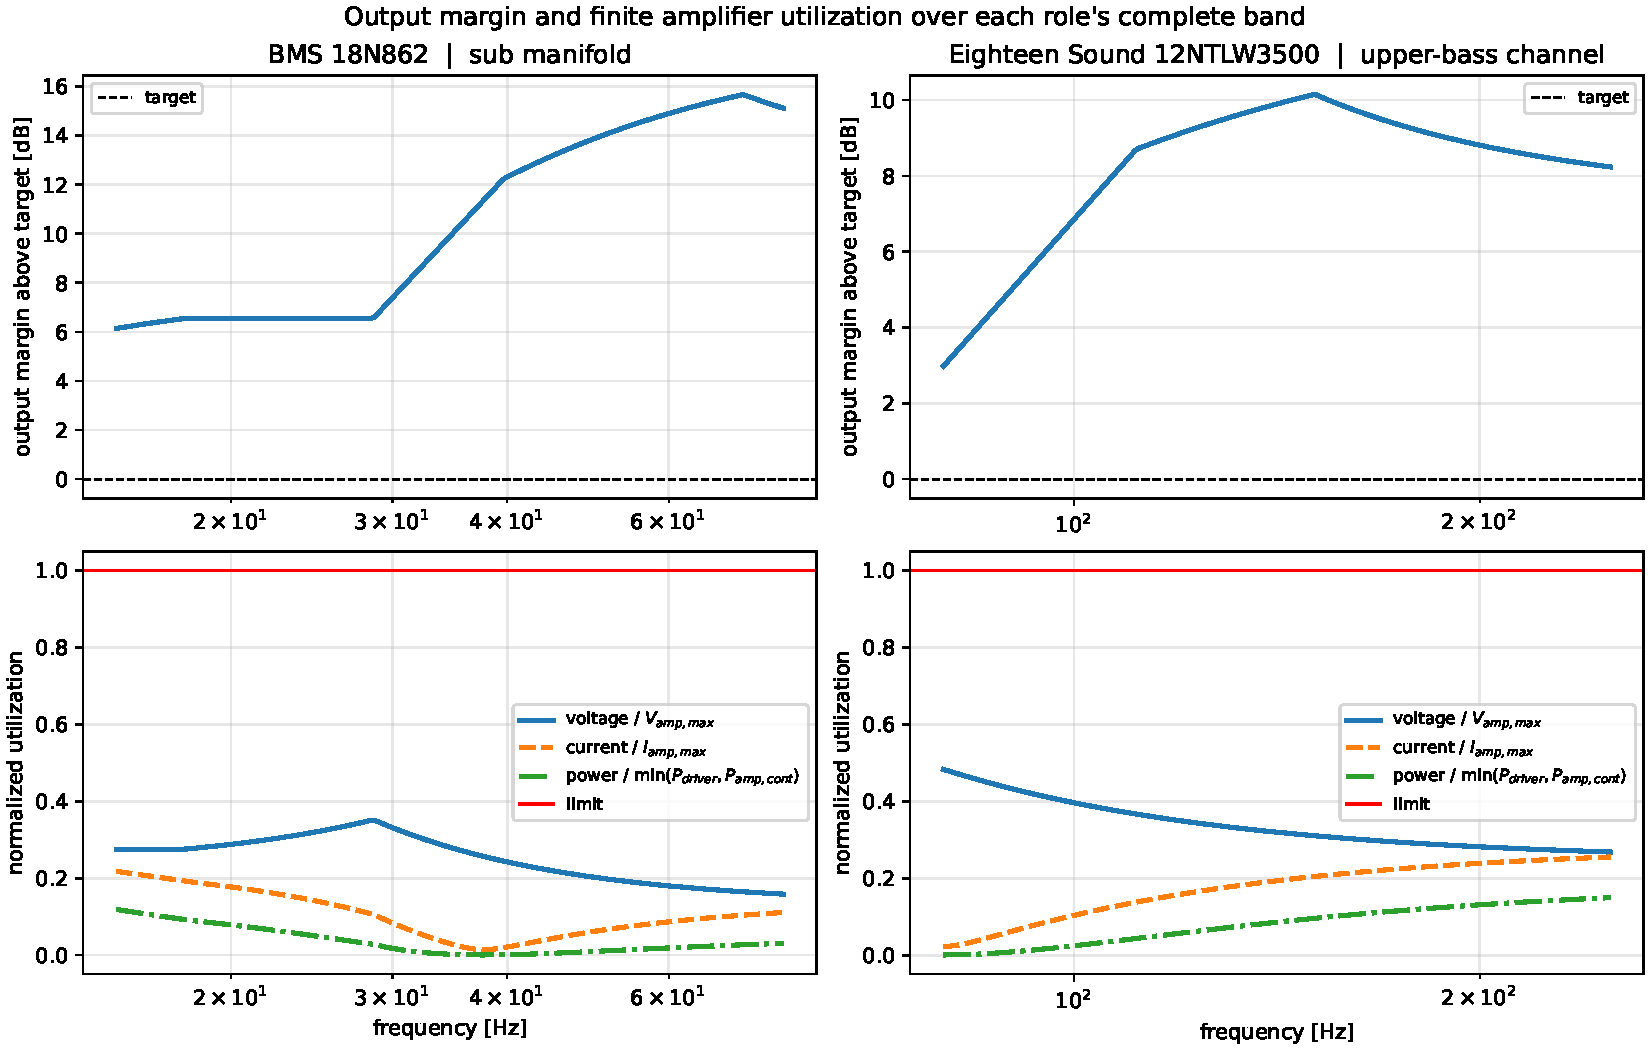
\includegraphics[width=0.96\textwidth]{figures/fig_output_electrical}
	\caption{Output margin and finite electrical utilization across both
	complete role bands.  The upper row compares the combined ceiling with
	the couch-area target.  The lower row shows per-driver voltage, current,
	and coil-power utilization against the declared limits.  The left
	column is the complete mono low-bass role; the right column is one
	independent upper-bass channel.}
	\label{fig:output-electrical}
\end{figure}

\section{Room-specific displaced-volume demand}
\label{sec:room}

\subsection{General room-transfer statement}

Let $H_{\mathrm{room}}(f)$ map source peak displaced volume to peak pressure
under a declared spatial reduction of the couch-area responses.  Then
\begin{equation}
	V_{\mathrm{dem}}(f)=
	\frac{\sqrt2\,p_t}{|H_{\mathrm{room}}(f)|},
	\qquad
	p_t=p_0\,10^{L_t/20}.
	\label{eq:demand-general}
\end{equation}
A measured transfer is preferred once a system or suitable source exists.
Before purchase, an analytical or parameterized room model can supply a
first sizing estimate.  Whatever transfer is used must preserve the same
reference basis throughout the role evaluation.

\subsection{Pressure-zone compliance with leakage}
\label{sec:room-pz}

Below the first axial mode, a net source displacement $\Delta V$ changes
room pressure approximately by the adiabatic compliance relation
\begin{equation}
	\Delta p=\frac{\rho_0c^2}{V_{\mathrm{room}}}\Delta V.
	\label{eq:room-compliance}
\end{equation}
Leakage prevents static pressure from being retained.  Representing it by a
first-order high-pass from source displacement to pressure gives
\begin{equation}
	H_{\mathrm{pz}}(s)=
	\frac{\rho_0c^2}{V_{\mathrm{room}}}
	\frac{s}{s+\omega_\ell},
	\label{eq:Hpz}
\end{equation}
and therefore
\begin{equation}
	|H_{\mathrm{pz}}(f)|=
	\frac{\rho_0c^2}{V_{\mathrm{room}}}
	\left[1+\left(\frac{f_\ell}{f}\right)^2\right]^{-1/2}.
	\label{eq:pzdyn}
\end{equation}
The ideal pressure-zone result is recovered for $f_\ell=0$.  Below the
leakage corner, the required displacement rises at approximately
\SI{6}{dB} per octave.

Above
$f_{\mathrm{pz}}\simeq c/(2L_{\max})$, the half-space radiation transfer is
\begin{equation}
	|H_{\mathrm{rad}}(f)|=
	\frac{\rho_0(2\pi f)^2}{2\pi r_{\mathrm{listen}}}.
	\label{eq:Hrad}
\end{equation}
To avoid an optimistic discontinuity below the first-mode boundary, the
implementation freezes the radiation demand at $f_{\mathrm{pz}}$ and takes
the larger demand:
\begin{equation}
	V_{\mathrm{dem}}(f)=
	\begin{cases}
	\dfrac{\sqrt2 p_t\,2\pi r_{\mathrm{listen}}}
	{\rho_0(2\pi f)^2},
	& f\ge f_{\mathrm{pz}},\\[2.2ex]
	\max\{V_{\mathrm{rad}}(f_{\mathrm{pz}}),V_{\mathrm{pz}}(f)\},
	& f<f_{\mathrm{pz}},
	\end{cases}
	\label{eq:Vdem}
\end{equation}
where
\begin{equation}
	V_{\mathrm{pz}}(f)=
	\frac{\sqrt2p_tV_{\mathrm{room}}}{\rho_0c^2}
	\sqrt{1+\left(\frac{f_\ell}{f}\right)^2}.
	\label{eq:Vpz}
\end{equation}

This is a low-frequency limiting model for a prepared room and a small
listening area.  The complete room remains distributed and multimodal.
Above the first axial mode, individual modes require fitted damped sections
or a measured transfer \cite{toole2006,makivirta2003}.  Room preparation is
therefore essential to the scenario: placement, damping, leakage control,
and soffit geometry are what make a low-order limiting model useful over its
declared range.

\subsection{Corner placement and sensitivity}

Combining \cref{eq:alignment} with the pressure-zone transition suggests
\begin{equation}
	F_c\simeq f_{\mathrm{pz}}
	\quad\Longleftrightarrow\quad
	\frac{F_s}{\Qts}\simeq
	\frac{f_{\mathrm{pz}}}{\Qtc^\ast}.
	\label{eq:Fsrule}
\end{equation}
This is a placement target, not a rejection rule by itself.  If the chosen
box cap forces $F_c$ above the target, the resulting correction boost is
evaluated by \cref{eq:Ereq,eq:Ireq,eq:Preq}.  If $F_c$ falls below it, a
response shelf can be reduced with a cut, at the cost of extra enclosure
volume.

\begin{figure}[htbp]
	\centering
	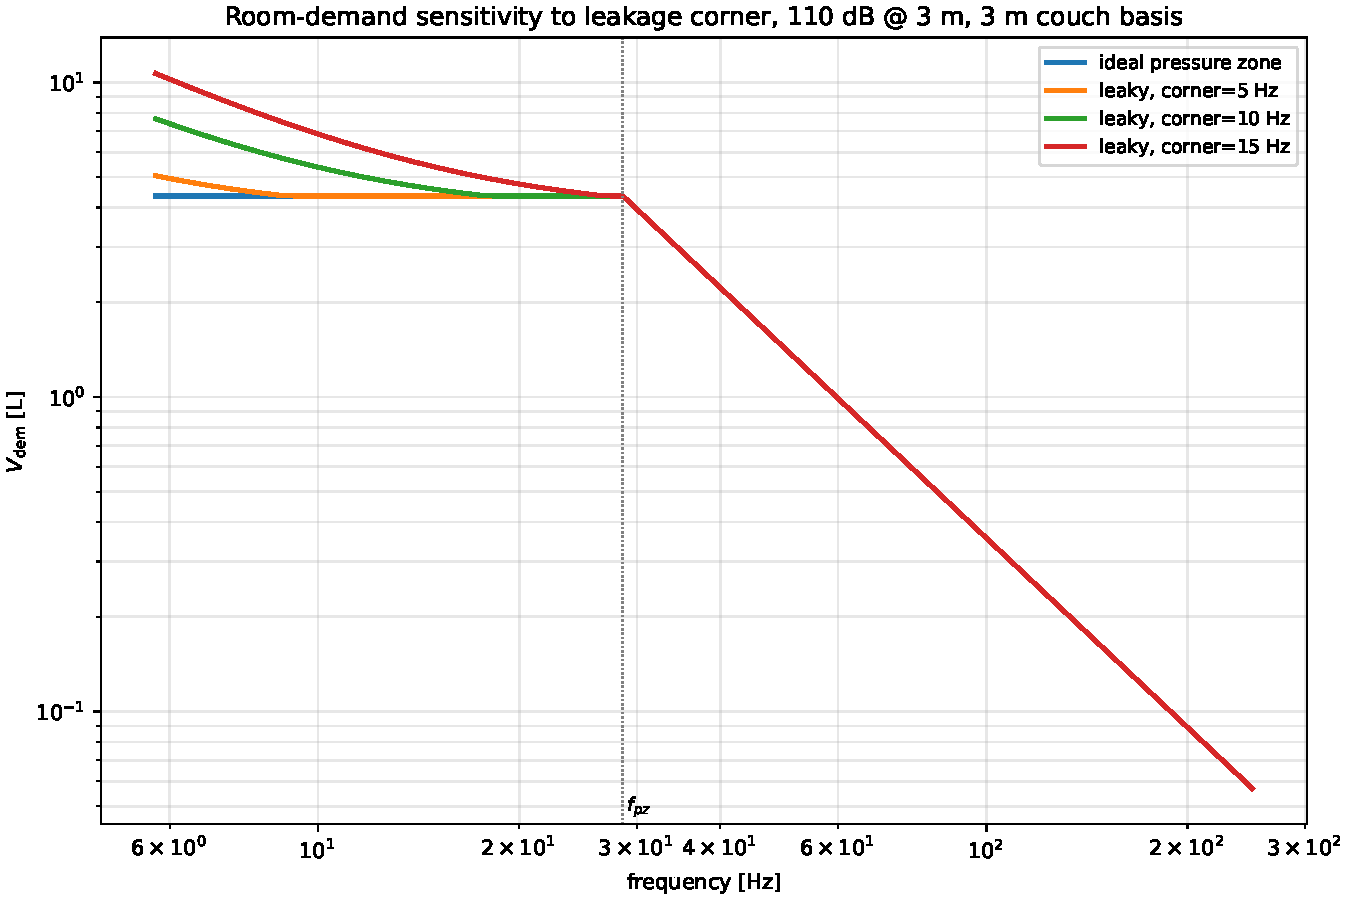
\includegraphics[width=0.88\textwidth]{figures/fig_room_sensitivity}
	\caption{Required peak displaced volume for the canonical target under
	the ideal pressure-zone case and several leakage corners.  Above
	$f_{\mathrm{pz}}$ all variants use the same radiation branch; below it,
	the assumed leakage controls the demand growth.}
	\label{fig:room-sensitivity}
\end{figure}

\begin{table*}[htbp]
\centering
\caption{Room-demand sensitivity to the leakage corner at the worst (lowest) sub-band frequency, 110 dB target at the 3 m listening-area basis ($V_{\mathrm{room}}$=60 m$^3$, $L_{\max}$=6 m). Required units use the selected Dayton Audio UMII18-22 sub driver's own $V_d$, rounded up to the nearest even count (opposed pairs permit first-order reaction-force cancellation under matched drive and mounting; the even count is a hard mechanical-layout constraint).}
\label{tab:room-sensitivity}
\begin{tabular}{lrrr}
\toprule
leakage corner & worst $V_{\mathrm{dem}}$ [L] & units at $X_{\max}$ & units at 80\% preferred\\
\midrule
ideal (0 Hz) & 4.36 & 2 & 2\\
5 Hz & 4.36 & 2 & 2\\
10 Hz & 4.57 & 2 & 2\\
15 Hz & 5.38 & 2 & 4\\
\bottomrule
\end{tabular}
\end{table*}


The table demonstrates why extension is conditional.  It depends on the
realized leakage corner, total available $\Vd$, the hard and preferred
excursion utilizations, and finite electrical headroom.  A nominal low
frequency is reported only where all gates hold.

\section{Finite-burst demand from the sealed ODE}
\label{sec:time}

\subsection{Why a numerical factor is needed}

A short waveform can require more displacement than a steady sinusoid that
reaches the same peak acceleration.  Free-mass arguments produce simple
constants only when the excitation frequency is far above $F_c$.  Both
roles here include frequencies near their box corners, where stiffness,
damping, start phase, and ring-down materially affect the result.

For a windowed burst
\begin{equation}
	e(t)=w(t)\sin(\omega t+\phi)
	\label{eq:burst}
\end{equation}
and the solution of \cref{eq:ode} from rest, define
\begin{equation}
	\boxed{
	C_{\mathrm{tr}}\left(
	\frac{f}{F_c},\Qtc,w,n,\phi
	\right)
	=
	\frac{\omega^2\max_{t\ge0}|x(t)|}
	{\max_{t\in\mathcal A}|\ddot x(t)|}}
	\label{eq:ctr}
\end{equation}
where $\mathcal A$ is the active burst interval.  The numerator includes
ring-down; the denominator is active-window acceleration, which sets peak
radiated pressure through \cref{eq:pofx}.  A steady sinusoid has
$C_{\mathrm{tr}}=1$ under the same normalization.

\subsection{Implemented numerical method}
\label{sec:time-method}

The reference implementation performs the following calculation for every
sampled role frequency:

\begin{enumerate}
	\item apply a unit-amplitude voltage burst to \cref{eq:ode};
	\item integrate displacement and velocity with fourth-order
	Runge--Kutta, using at least 96 integration steps per relevant cycle;
	\item sample eight phases uniformly over $0\le\phi<2\pi$, which includes
	sine and cosine starts;
	\item retain active-window peak acceleration and active-window rms
	voltage and current;
	\item continue the zero-input integration for eight envelope time
	constants and retain peak displacement through the ring-down;
	\item scale the unit response so its active acceleration equals
	$\omega^2X_{\mathrm{dem}}$, then compute displacement, voltage, current,
	and coil power;
	\item retain the worst result over phase and then over the sampled role
	band.
\end{enumerate}

The canonical waveform is one rectangular cycle.  The figure also shows
Hann-windowed cases to expose waveform dependence, but those curves do not
replace the declared canonical test.  Discretization is part of the
implementation and is covered by the numerical test suite; the waveform
family remains an engineering input.

\begin{figure}[htbp]
	\centering
	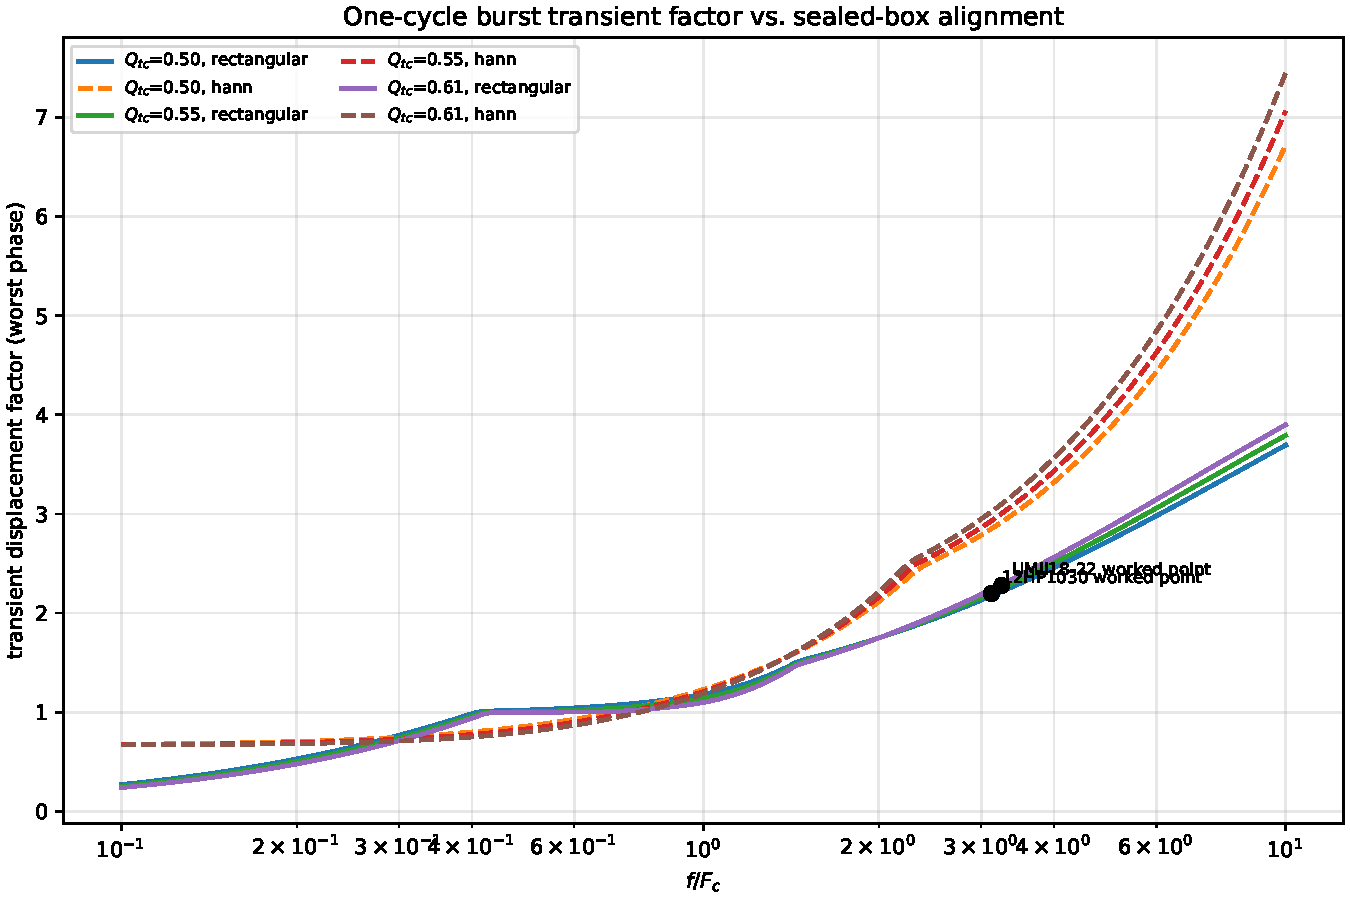
\includegraphics[width=0.9\textwidth]{figures/fig_transient_factor}
	\caption{Numerically evaluated $C_{\mathrm{tr}}$ versus normalized
	frequency for several alignments and windows, retaining the worst start
	phase.  The worked-system operating points are marked.  The variation
	near $F_c$ is why the procedure solves the ODE rather than applying one
	fixed burst constant.}
	\label{fig:transient}
\end{figure}

\subsection{Transient gates}

At the target pressure,
\begin{equation}
	\xi_x^{\mathrm{tr}}=
	\frac{\max_t|x(t)|}{\Xmax}
	=C_{\mathrm{tr}}\frac{X_{\mathrm{dem}}}{\Xmax}.
	\label{eq:xitr}
\end{equation}
The equivalent transient excursion ceiling on B1 is
\begin{equation}
	\mathrm{SPL}_{\mathrm{L,tr}}(f)=
	\mathrm{SPL}_{\mathrm L}(f)
	-20\log_{10}C_{\mathrm{tr}}(f).
	\label{eq:spltr}
\end{equation}
The hard transient checks per driver are
\begin{equation}
	\boxed{
	\xi_x^{\mathrm{tr}}\le1,\quad
	E_{\mathrm{tr}}\le E_{\mathrm{amp}},\quad
	I_{\mathrm{tr}}\le I_{\mathrm{amp}},\quad
	P_{\mathrm{tr}}\le P_{\mathrm{amp,burst}}.}
	\label{eq:transient-gates}
\end{equation}
Active-window rms values are used for the electrical burst quantities.  The
continuous driver and amplifier limits remain checked against steady demand.

\section{Separately reported nonlinear-risk and implementation indicators}
\label{sec:risk}

The method reports
\begin{equation}
	\mathbf r=
	\left(
	\xi_x,\xi_x^{\mathrm{tr}},d_{\mathrm D},
	\xi_{\mathrm{box}},\xi_P,\xi_{\mathrm{amp}},
	f_{\mathcal B,\mathrm h}/f_L,V_{\mathrm b}^{\mathrm{tot}}
	\right).
	\label{eq:riskvec}
\end{equation}
These quantities have different physical origins and perceptual meanings.
They remain separate in tables, plots, Pareto objectives, and policy keys.

\subsection{Steady and transient excursion utilization}

\begin{equation}
	\xi_x=\max_{f\in\mathcal B}
	\frac{X_{\mathrm{dem}}(f)}{\Xmax},
	\qquad
	\xi_x^{\mathrm{tr}}=
	\max_{f\in\mathcal B}
	\frac{X_{\mathrm{tr}}(f)}{\Xmax}.
	\label{eq:xi}
\end{equation}
$\Xmax$ provides the hard boundary.  The preference
$\max(\xi_x,\xi_x^{\mathrm{tr}})\le0.80$ reserves displacement margin.
The procedure does not reconstruct $Bl(x)$ or suspension coefficients from
these ratios.

\subsection{Doppler first-sideband ratio}

For each role, let
\begin{equation}
	X_{\mathcal B}=
	\max_{f\in\mathcal B}X_{\mathrm{dem}}(f)
	\label{eq:Xband}
\end{equation}
and use that role's own upper band edge $f_{\mathcal B,\mathrm h}$.  The
phase-modulation index is
\begin{equation}
	m=2\pi f_{\mathcal B,\mathrm h}X_{\mathcal B}/c.
	\label{eq:doppler-m}
\end{equation}
For small $m$, either first sideband has amplitude relative to the carrier
\begin{equation}
	\boxed{
	d_{\mathrm D}=\frac{J_1(m)}{J_0(m)}
	\simeq\frac{m}{2}
	=\frac{\pi f_{\mathcal B,\mathrm h}X_{\mathcal B}}{c}.}
	\label{eq:doppler}
\end{equation}
The canonical budget is $d_{\mathrm D}\le0.02$.  The value is reported for
both roles; it is a hard gate for the upper-bass role in the implemented
policy and a reported ordering indicator for the low-bass role.  Splitting
the bands prevents a low-bass radiator from modulating upper-bass content on
that same cone, but finite crossover overlap and self-modulation within each
role remain.

\subsection{Box-spring indicator}

For an adiabatic gas, expanding pressure versus fractional volume change
gives an asymmetric leading term.  Weighting it by the box fraction of the
total stiffness gives
\begin{equation}
	\boxed{
	\xi_{\mathrm{box}}\simeq
	\frac{\gamma+1}{4}
	\frac{V_{\mathrm{dem}}}{N\Vb}
	\left(1-\frac{\Qts^2}{\Qtc^2}\right).}
	\label{eq:boxHD}
\end{equation}
This is an enclosure indicator.  It decreases with larger volume and with a
lower effective polytropic exponent from suitable filling.  It is not
combined arithmetically with excursion or Doppler quantities.

\subsection{Electrical, thermal, enclosure, and inductive indicators}

\begin{align}
	\xi_P&=
	\max_{f\in\mathcal B}
	\frac{P_{\mathrm{req}}(f)}{\Pmax},
	\label{eq:xip}\\
	\xi_{\mathrm{amp}}&=
	\max\left\{
	\frac{\max(E_{\mathrm{req}},E_{\mathrm{tr}})}{E_{\mathrm{amp}}},
	\frac{\max(I_{\mathrm{req}},I_{\mathrm{tr}})}{I_{\mathrm{amp}}},
	\frac{\max P_{\mathrm{req}}}{P_{\mathrm{amp,cont}}},
	\frac{\max P_{\mathrm{tr}}}{P_{\mathrm{amp,burst}}}
	\right\}.
	\label{eq:xiamp}
\end{align}
$\xi_P$ is a loading warning, not a coil-temperature model.  The inductive
ratio uses
\begin{equation}
	f_L=\frac{\Re}{2\pi\Le}.
	\label{eq:fL}
\end{equation}
Because $\Le$ is neither constant nor always published, this is deliberately
a rough screen.  Total role enclosure volume is retained as a packaging
quantity:
\begin{equation}
	V_{\mathrm b}^{\mathrm{tot}}=N\Vb.
	\label{eq:vbtot}
\end{equation}

\section{Selection, Pareto ranking, and implementation}
\label{sec:procedure}

\subsection{Alignment selection}

For a candidate corner rate $F_s/\Qts$, the Q that would place the box
corner exactly at the role target $f_{\mathrm target}$ is
\begin{equation}
	\Qtc^{\mathrm target}=
	\frac{f_{\mathrm target}}{F_s/\Qts}.
	\label{eq:qtarget}
\end{equation}
The implementation chooses
\begin{equation}
	\Qtc^{\mathrm desired}=
	\min\left\{\Qtc^\ast,\Qtc^{\mathrm target}\right\},
	\label{eq:qdesired}
\end{equation}
where $f_{\mathrm target}=f_{\mathrm{pz}}$ for low bass and
$f_{\mathrm target}=f_{\mathrm{sp}}$ for upper bass.  It computes the
required \cref{eq:boxvolume}; if that volume exceeds
\begin{equation}
	\Vb^{\mathrm cap}=
	\min\left\{10\Vas,
	\frac{\SI{1.0}{\cubic\meter}}{N}\right\},
	\label{eq:boxcap}
\end{equation}
the cap is used and the realized $\Qtc$ is recalculated.  A realized
$\Qtc>0.55$ fails.

\subsection{Band evaluation}

Steady quantities use a logarithmic 121-point grid plus relevant corner
frequencies.  Transient quantities use a smaller logarithmic grid because
each frequency requires repeated ODE integrations; band edges and relevant
corners are again included.  At each point the implementation evaluates the
room demand, per-driver displacement, steady electrical requirements, and
finite-burst requirements.  Each maximum is retained with its binding
frequency.  This is a declared numerical approximation over a finite band,
not an assertion that an unsampled narrow anomaly cannot exist in a physical
driver.

\subsection{Hard gates}
\label{sec:hard-gates}

A candidate is rejected if any of the following occurs:

\begin{itemize}
	\item realized $\Qtc$ exceeds its ceiling;
	\item steady or transient displacement exceeds $\Xmax$;
	\item steady voltage, current, driver dissipation, or amplifier
	continuous power exceeds its limit;
	\item burst voltage, current, or amplifier burst power exceeds its limit;
	\item reported $f_L$ is below the role upper edge;
	\item the upper-bass Doppler first-sideband ratio exceeds $0.02$.
\end{itemize}

The preferred $0.80$ excursion marker is not in this list.  Every rejection
stores its reason; every missing or derived field stores a note.

\subsection{Role-specific Pareto fronts}

For low bass, the core minimization vector is
\begin{equation}
	\left(
	\max\{\xi_x,\xi_x^{\mathrm{tr}}\},
	\xi_{\mathrm{amp}},
	V_{\mathrm b}^{\mathrm{tot}}
	\right).
	\label{eq:pareto-sub}
\end{equation}
For upper bass it is
\begin{equation}
	\left(
	\max\{\xi_x,\xi_x^{\mathrm{tr}}\},
	d_{\mathrm D},
	\xi_{\mathrm{amp}},
	V_{\mathrm b}^{\mathrm{tot}}
	\right).
	\label{eq:pareto-upper}
\end{equation}
Candidate A dominates candidate B only when A is no worse in every component
and strictly better in at least one.  Removing the current non-dominated set
and repeating assigns successive fronts.  Public front numbers begin at one.
The full vector in \cref{eq:riskvec} remains available even when a component
is not a core Pareto coordinate.

\subsection{Lexicographic policy within each front}

The low-bass order is:
\begin{enumerate}
	\item minimum worst transient-or-steady excursion;
	\item minimum steady excursion;
	\item minimum Doppler first-sideband ratio;
	\item minimum worst driver/electrical utilization;
	\item minimum box-spring indicator;
	\item minimum total role box volume;
	\item minimum preferred unit count, then a stable label tie-break.
\end{enumerate}

The upper-bass order is:
\begin{enumerate}
	\item prefer candidates meeting the $0.80$ excursion marker;
	\item maximize $\eta_0\Pmax$;
	\item prefer reported, valid inductance over unresolved inductance;
	\item maximize $f_L$;
	\item minimize excursion, electrical utilization, and box volume;
	\item apply a stable label tie-break.
\end{enumerate}

A system pair is feasible only if both role evaluations are feasible.  Pairs
are compared first by low-bass front, then upper-bass front, then the two
role policy keys, physical driver count, and total enclosure volume.  Role
risks remain separate.

\subsection{Candidate population and privacy boundary}
\label{sec:database}

The aggregate population is a separately obtained VituixCAD community
driver-database export.  The repository does not contain that source or any
row-level derivative.  The public manifest records its SHA-256 digest,
parser entry point, required fields, filters, retained/skipped counts, role
counts, canonical scenario, and the exact public selected-driver records.

\begin{figure}[htbp]
	\centering
	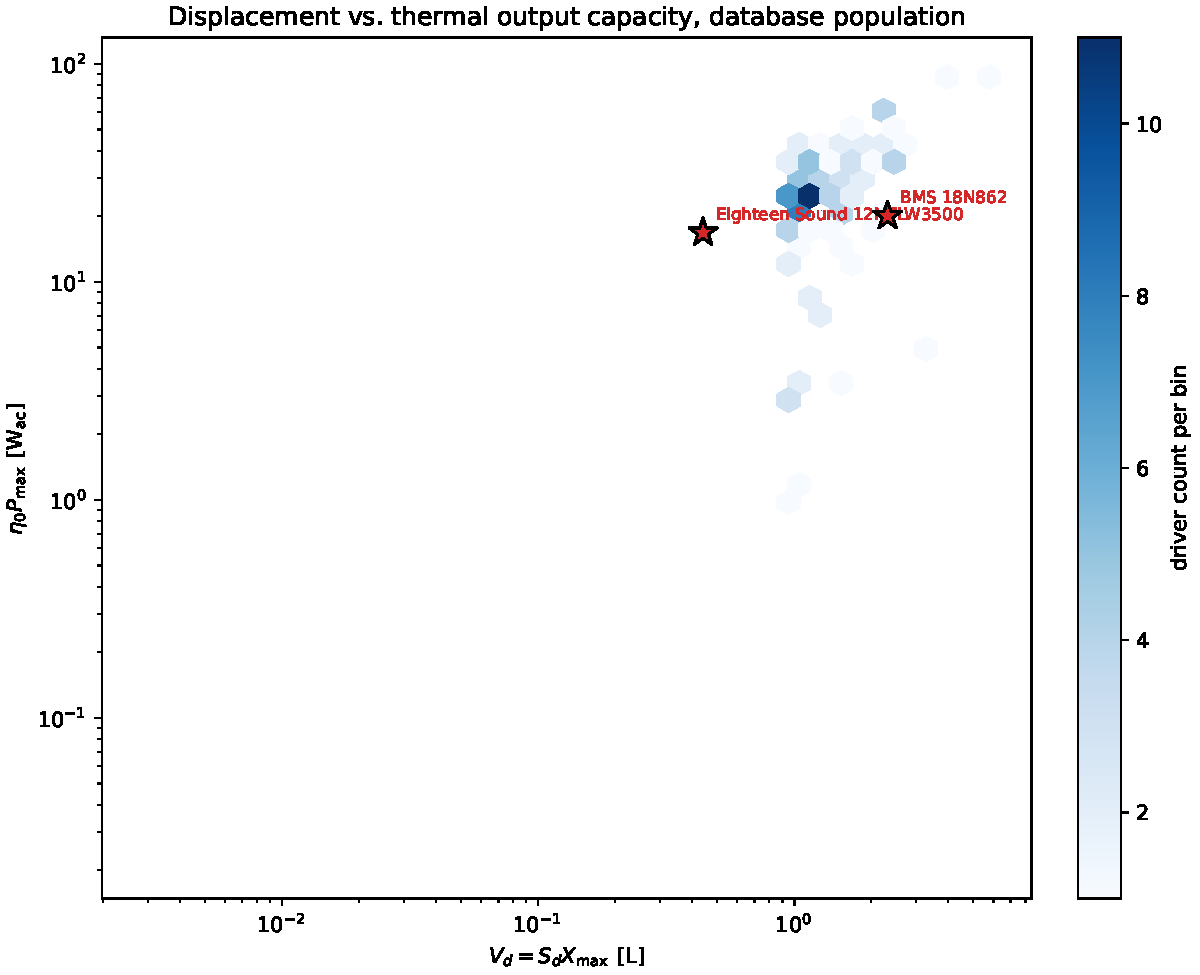
\includegraphics[width=0.88\textwidth]{figures/fig_database_pareto}
	\caption{Binned aggregate population in the
	$(\Vd,\eta_0\Pmax)$ plane.  Binning avoids disclosure of individual
	private-source rows.  The two public worked-example records are marked.}
	\label{fig:database-pareto}
\end{figure}

\begin{figure}[htbp]
	\centering
	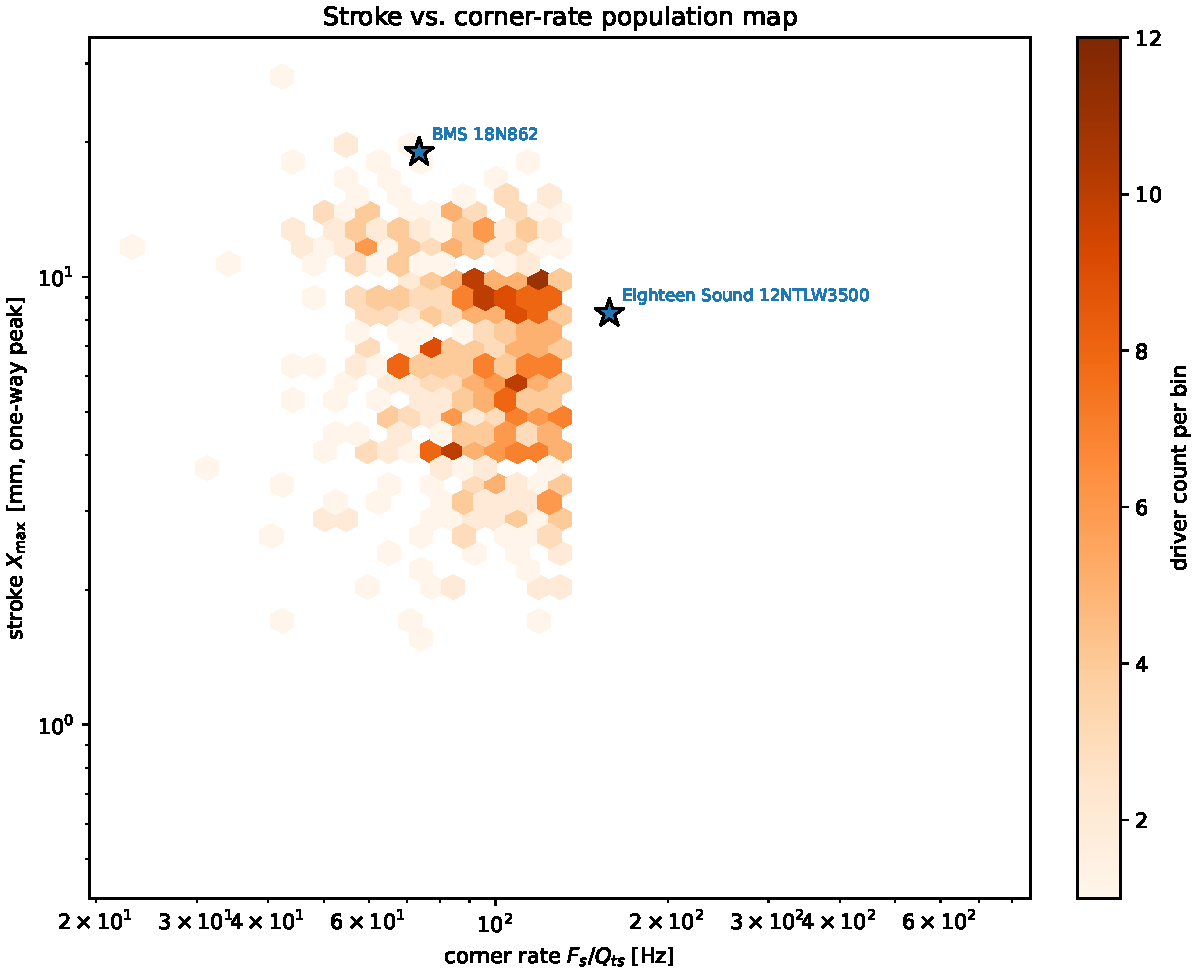
\includegraphics[width=0.88\textwidth]{figures/fig_corner_population}
	\caption{Aggregate stroke versus exact corner-rate population.  The plot
	shows the empirical spread of available records and the locations of the
	public worked-example drivers.  It is descriptive population evidence,
	not a physical exclusion curve.}
	\label{fig:corner-population}
\end{figure}

\begin{table*}[htbp]
\centering
\caption{Private driver-database evidence summary at the worked unit counts (aggregate counts only. The accompanying manifest supplies the full source hash, parser, and filter definitions).}
\label{tab:database-summary}
\begin{tabular}{lr}
\toprule
quantity & value\\
\midrule
source hash (SHA-256, first 12 hex) & \texttt{0a5edbd1868e}\\
retained rows & 1342\\
skipped rows (missing required fields) & 537\\
sub-manifold role candidates (15--21in) & 246\\
sub-manifold role feasible (2 total) & 1\\
sub-manifold role Pareto front & 1\\
upper-bass role candidates (8--15in) & 592\\
upper-bass role feasible (1/channel) & 146\\
upper-bass role Pareto front & 41\\
both role tests feasible at worked counts (size-unrestricted) & 1\\
\bottomrule
\end{tabular}
\end{table*}


The size-unrestricted aggregate includes candidates feasible in both bands.
The selected roles nevertheless occupy different parts of the observed
population under the role size filters, targets, packaging limits, and
policy.  This is an empirical scenario result, not a prohibition on a
single-driver design.

\subsection{Robustness as decision stability}
\label{sec:robustness}

The pipeline reruns rankings with $\Xmax$ shifted by $\pm25\%$, $\Pmax$
shifted by $\pm\SI{3}{dB}$, alternative leakage corners, and alternative
reasonable ordering priorities.  It reports top-$k$ shortlist overlap:
\begin{equation}
	R_k=\frac{|S_k^{(0)}\cap S_k^{(v)}|}{k}.
	\label{eq:robustness}
\end{equation}

\begin{figure}[htbp]
	\centering
	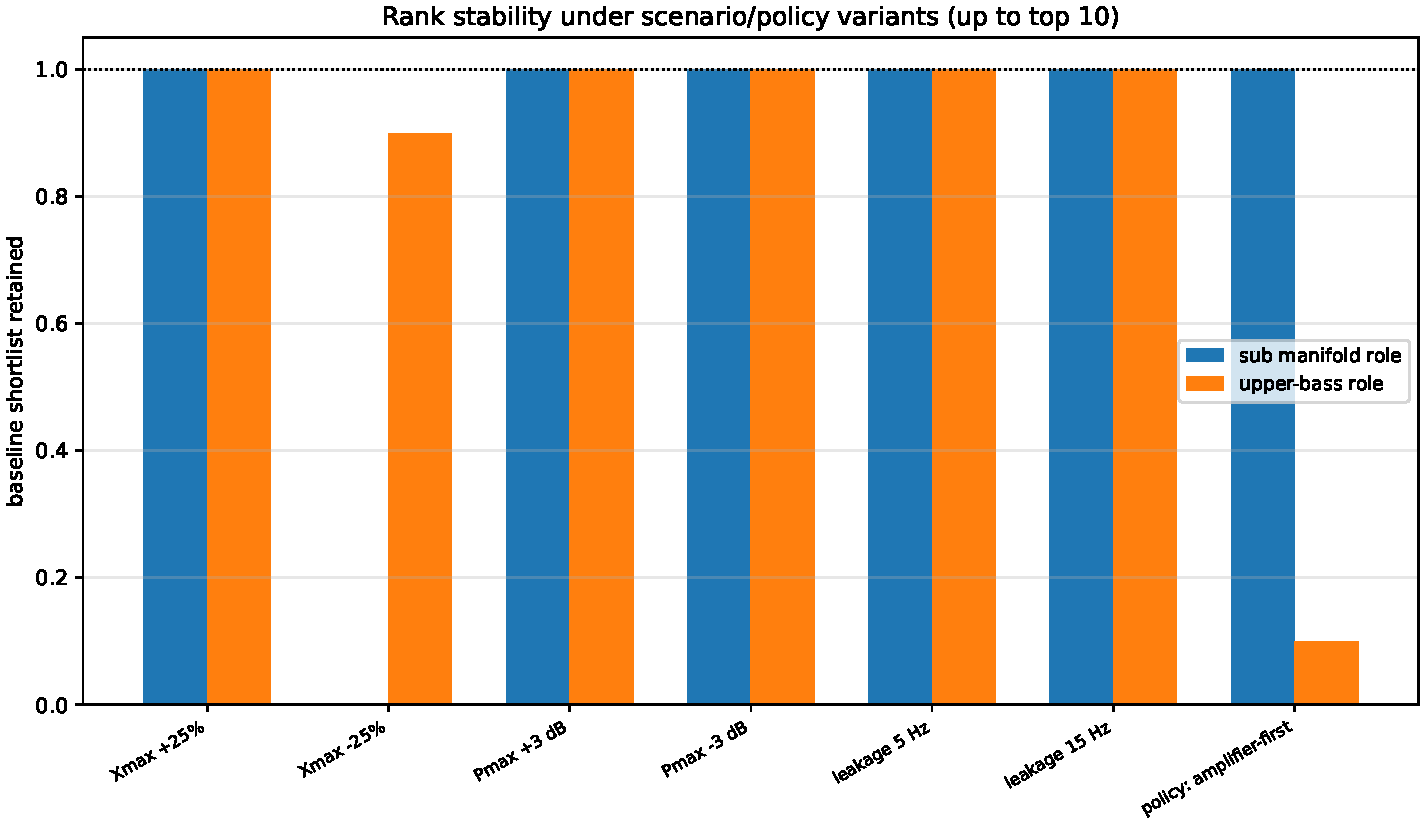
\includegraphics[width=0.9\textwidth]{figures/fig_rank_robustness}
	\caption{Top-$k$ overlap with the baseline under datasheet, room, and
	policy variants.  High overlap means the practical shortlist is stable
	to that perturbation; low overlap identifies a provisional ordering.}
	\label{fig:rank-robustness}
\end{figure}

This analysis tests decision stability only.  It does not validate physical
large-signal behaviour, audibility, or the room model.

\section{Worked public-datasheet system}
\label{sec:example}

\subsection{Low-bass manifold}

The selected low-bass system uses four BMS 18N862 drivers in two
mechanically opposed pairs.  The opposed layout permits first-order
reaction-force cancellation only when drive, drivers, and mounting are
matched.  Unit variation, gain/phase mismatch, and mounting tolerance leave
residual force.  Each physical driver has its own amplifier channel.

The \SI{110}{dB} target is the total manifold target from
\SIrange{15}{80}{\hertz}.  The box cap binds at
\SI{250}{\liter} per driver, filling the \SI{1.0}{\cubic\meter} low-bass
role allowance.  The resulting alignment is approximately
$\Qtc=0.512$ and $F_c=\SI{37.6}{\hertz}$.  Because $F_c$ is above
$f_{\mathrm{pz}}$, the finite-band correction cost is included in every
electrical and displacement result.

\subsection{Independent upper-bass channels}

Each stereo channel uses one Eighteen Sound 12NTLW3500-8.  The public
manufacturer one-way $\Xmax=\SI{8.3}{\milli\meter}$ is used.  A
\SI{35.2}{\liter} enclosure gives approximately
$\Qtc=0.506$ and $F_c=\SI{80}{\hertz}$.  Each channel must independently
meet \SI{105}{dB} from \SIrange{80}{250}{\hertz}.

\subsection{Gate results}

Under the \SI{10}{\hertz} leakage model, the low-bass displaced-volume
demand is largest at \SI{15}{\hertz}.  The generated room-sensitivity table
gives \SI{4.57}{\liter} peak for the complete manifold, or about
\SI{1.14}{\liter} per driver before division by piston area.

The generated worked table is the authoritative rounded summary.  The
low-bass role reaches approximately $0.49$ steady and $0.51$ transient
excursion utilization.  Its worst steady requirements are approximately
\SI{31.7}{\volt} rms, \SI{3.3}{\ampere} rms, and \SI{59}{\watt} per
driver.  The upper-bass role reaches approximately $0.71$ steady and
$0.83$ transient excursion utilization, with approximately
\SI{43.5}{\volt} rms, \SI{3.8}{\ampere} rms, and \SI{75}{\watt} at the
respective worst frequencies.  The latter transient utilization crosses the
preferred marker but remains below the hard boundary.

\begin{figure}[htbp]
	\centering
	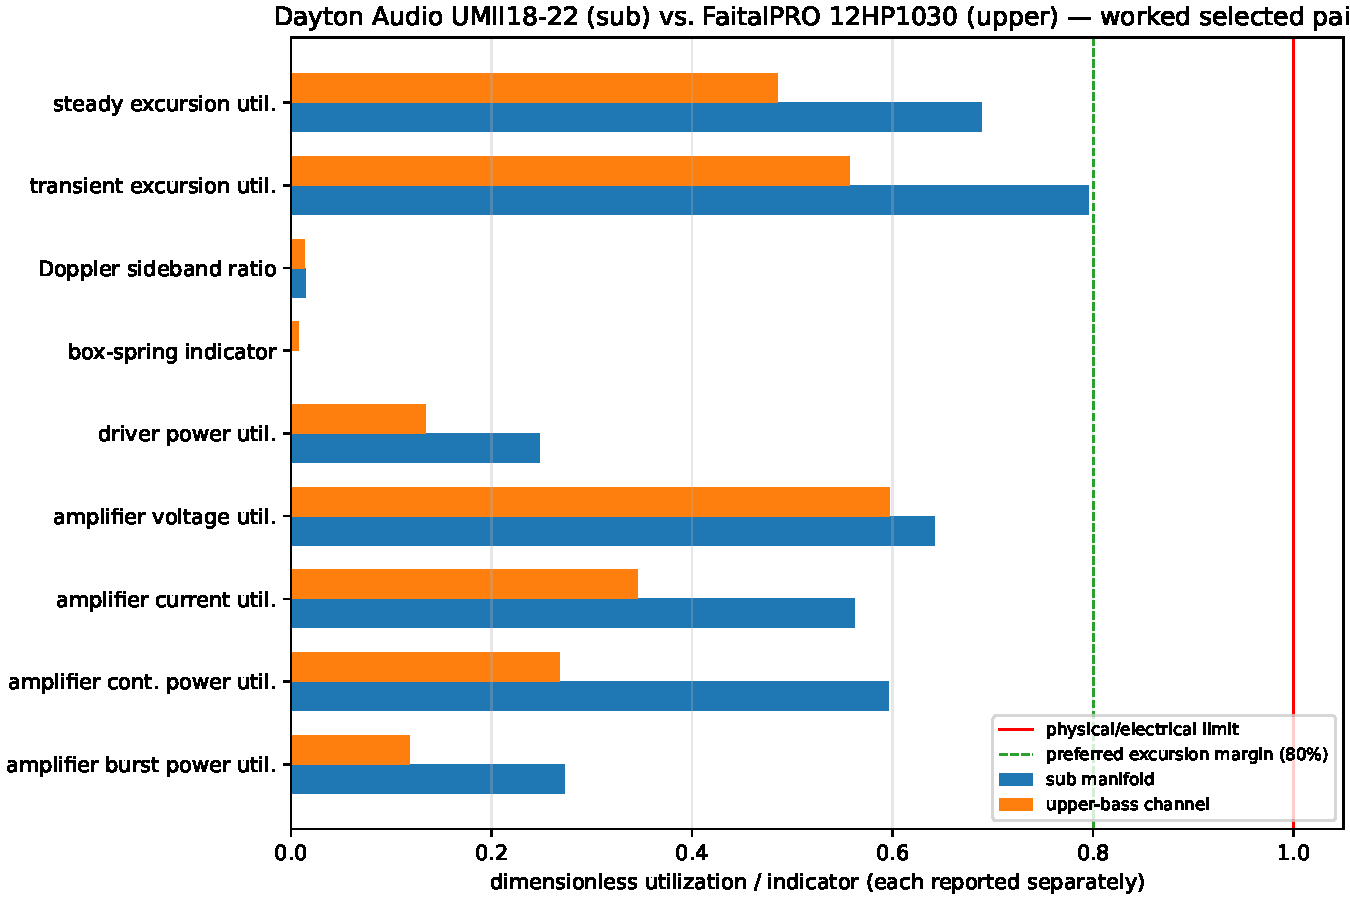
\includegraphics[width=0.9\textwidth]{figures/fig_worked_system}
	\caption{Separately reported worked-system indicators for the complete
	mono manifold and one upper-bass stereo channel.  The hard boundary and
	preferred excursion marker are shown without combining unlike
	quantities.}
	\label{fig:worked-system}
\end{figure}

\begin{table*}[htbp]
\centering
\caption{Worked selected pair: Dayton Audio UMII18-22 (mono sub manifold, 2 identical units in an even, symmetrically opposed pairing -- permitting first-order reaction-force cancellation under matched drive and mounting; the even count is a hard mechanical-layout constraint, not a ranking-policy preference -- each with its own amplifier channel, aggregate target 110 dB for the manifold, not per driver) and FaitalPRO 12HP1030 (upper-bass, one unit per independent stereo channel, target 105 dB per channel). Pareto front number is one-based and is against this report's frozen private-database candidate pool for each role.}
\label{tab:worked-pair}
\small
\begin{tabular}{p{4.0cm}p{5.1cm}p{5.1cm}}
\toprule
 & Dayton UMII18-22 (sub) & FaitalPRO 12HP1030 (upper)\\
\midrule
public source & Dayton Audio official UMII18-22 specification sheet & FaitalPRO official 12HP1030 product data (8 ohm)\\
role, units & mono sub manifold, 2x (even, opposed pairs for first-order force cancellation when matched), aggregate target 110 dB for the manifold & stereo upper-bass, 1x per channel, target 105 dB per channel\\
$V_d$ per driver [L] & 3.32 & 0.64\\
$\eta_0 P_{\max}$ [W$_{\mathrm{ac}}$] & 4.63 & 10.32\\
$F_s$ / $Q_{ts}$ & 22 Hz / 0.530 & 45 Hz / 0.303\\
$f_L=\Re/2\pi\Le$ [Hz] & 581 & 589\\
box per driver: $V_b$, $F_c$ & 993 L, 24.6 Hz & 16.6 L, 80.0 Hz\\
$Q_{tc}$ & 0.592 & 0.539\\
worst steady excursion util. & 0.69 & 0.48\\
worst transient excursion util. & 0.80 & 0.56\\
worst voltage [V rms @ Hz] & 56.9 @ 28.6 & 53.7 @ 80.0\\
worst current [A rms @ Hz] & 8.4 @ 80.0 & 5.2 @ 250.0\\
worst power [W @ Hz] & 298 @ 80.0 & 134 @ 250.0\\
Pareto front / status & 1 / feasible & 1 / feasible\\
\bottomrule
\end{tabular}
\end{table*}


Three conclusions follow within this scenario.  First, box volume fixes the
low-bass alignment and correction demand, whereas transient excursion is the
tighter upper-bass concern.  Second, all finite per-driver amplifier gates
remain satisfied across both complete bands.  Third, the recommendation is
conditional on the room leakage model; the available low-bass margin absorbs
the declared sensitivity range but remains finite.

\section{Scoped sealed-versus-vented comparison}
\label{sec:vented}

\subsection{Order and limiting behaviour}

A vented enclosure adds port acoustic mass and resistance to the driver and
box compliance, producing a fourth-order alignment \cite{small1973vented}.
Around tuning it can deliver greater acoustic output per cone displacement
and greater electrical efficiency than a same-volume sealed system.  Those
are strong advantages when amplifier power or passband efficiency binds.

Below tuning, however, port and cone volume velocities no longer combine in
the same protective way.  Cone excursion rises rapidly unless a suitable
high-pass filter limits programme content.  A practical vented design
therefore adds that filter and evaluates its voltage, current, excursion,
port, and group-delay consequences.  This is a manageable engineering task,
but it differs from the sealed model in which the air spring bounds
low-frequency displacement for a bounded voltage input down to dc.

\subsection{Room integration}

The sealed low-frequency response has a second-order high-pass asymptote,
which can approximately complement the pressure-zone transition over the
declared prepared-room range.  A vented system rolls off more steeply below
tuning, so matching it to the same room and extension objective requires a
different alignment and protective-filter calculation.  Neither topology
removes the need for measured in-room verification above the first axial
mode.

\subsection{Port and passive-radiator constraints}

Near tuning, port volume velocity supplies much of the output.  A useful
first estimate for mean port speed at target pressure $p_t$ is
\begin{equation}
	v_{\mathrm{port}}\simeq
	\frac{2\pi r_{\mathrm{listen}}p_t}
	{\rho_0\omega_bS_{\mathrm{port}}}.
	\label{eq:portvelocity}
\end{equation}
Port compression, vortex shedding, turbulence noise, and end correction
then depend on geometry and level \cite{salvatti2002,vanderkooy1998}.
Large or multiple flared ports reduce velocity but require volume and baffle
area.  Passive radiators remove the port-flow mechanism while retaining the
additional resonant degree of freedom and below-tuning excursion issue.

\subsection{Why sealed loading is retained here}

The canonical manifold already uses multiple actively driven units for
displacement and opposed-pair force reduction.  Under the generated worked
result, enclosure volume and excursion bind before amplifier power.
Sealed loading consequently offers a compact modelling and protection
advantage for this application: one bounded-excursion second-order plant per
driver, no port geometry, and a direct fit to the declared room-sizing
procedure.  Different constraints---particularly tighter amplifier power,
greater required sensitivity near tuning, or a room without useful
pressure-zone support---can favour vented or passive-radiator loading.  The
present ranking equations would then need to be rederived for that plant.

\section{Limitations and required validation}
\label{sec:limits}

\begin{enumerate}
	\item The driver model is small-signal and LTI.  It omits measured
	$Bl(x)$, $K_{\mathrm{ms}}(x)$, inductance modulation, hysteresis, creep,
	and suspension heating.
	\item Published $\Xmax$, $\Pmax$, and $\Le$ fields have mixed conventions
	and unknown production spread.  Robustness analysis can reveal
	sensitivity to those fields but cannot correct their definitions.
	\item The thermal check is dissipation-based.  It does not predict coil
	temperature, magnet heating, time-varying resistance, or compression.
	\item The rigid-piston radiation model omits directivity transition,
	cone breakup, baffle details, mutual radiation impedance, and near-field
	effects.
	\item The room model is a limiting compliance-plus-leakage description
	below the first axial mode.  Above that range, measured transfers or
	fitted modal sections are required.
	\item The couch-area objective must be implemented as a declared
	reference or spatial aggregation.  The current analytical example does
	not establish uniformity throughout the area.
	\item DSP correction is constrained by noise, latency, finite filter
	length, spatial variation, headroom, and model error.
	\item Reaction-force cancellation is first order and depends on matched
	drive and mounting.
	\item Aggregate database results inherit mixed manufacturer conventions,
	unknown age, and unknown current availability.  They describe the frozen
	snapshot, not the current market.
	\item The robustness plot measures stability of the decision procedure,
	not correctness of the physical proxies.
	\item No controlled subjective comparison with a diffuse-field,
	multi-seat, vented, or multichannel system is reported.
\end{enumerate}

The most important future work is therefore measured validation at three
levels:

\begin{enumerate}
	\item public large-signal measurements on a comparable subset of drivers,
	testing whether proxy-based pairwise ordering agrees with measured
	headroom;
	\item a measured transfer over the prepared couch area replacing the
	analytical room model;
	\item a built-system test of frequency response, phase/delay integration,
	maximum output, voltage/current, compression, distortion spectra,
	reaction force, and spatial variation.
\end{enumerate}

\section{Reproducibility and data boundary}
\label{sec:availability}

The implementation is in \path{src/audioshape/}, with scenario construction
in \path{scenario.py}, physical relations in \path{physics.py}, ranking in
\path{ranking.py}, and serializable recipe loading in \path{recipe.py}.
The canonical manifest is
\path{papers/26325/data/driver_database_manifest.json}.  It records the
private source hash and metadata, aggregate counts, and exact public SI
records for the selected BMS and Eighteen Sound drivers.  The source URLs are
manufacturer URLs in that manifest.

The private VituixCAD export is neither included nor reconstructable from the
published package.  Only its digest, parser/filter metadata, aggregate
counts, and non-row-level plots are public.  The generated figures and tables
used by both manuscripts are committed under
\path{papers/26325/figures/} and \path{papers/26325/tables/}.

The author develops loudspeaker design software commercially at SenseMagic.
The reference implementation, generated evidence, and this explanatory
companion are available from the project repository
\cite{audioshape-preprint}.

\section{Conclusion}
\label{sec:conclusion}

For the declared prepared-room, soffit-mounted, small-area stereo
architecture, the method provides a reproducible path from public datasheet
records to separate low-bass and upper-bass shortlists.  It retains the
classical sealed ODE, alignment line, displacement and dissipation ceilings,
$f_x$ equivalence, room-demand derivation, and full-band electrical
requirements; it adds a declared numerical finite-burst test and a
non-compensatory decision policy.

The canonical worked system uses four BMS 18N862 drivers in two opposed pairs
for the mono manifold and one Eighteen Sound 12NTLW3500-8 per upper-bass
stereo channel.  Under the stated room model, box limits, targets, and
per-driver electronics, both roles satisfy their hard gates.  The selected
records occupy different empirical regions and have different binding
constraints, but that observation is specific to the frozen population and
scenario.

The procedure's strongest claim is practical: it makes assumptions,
reference bases, correction cost, electrical limits, uncertainty, and
ranking priorities inspectable before purchase.  Physical confidence still
requires large-signal driver measurement, a measured prepared-room transfer,
and verification of the built system.

\appendix

\section{Derivation of the leaky pressure-zone transfer}
\label{app:room-derivation}

Let room compliance be
\begin{equation}
	C_{\mathrm a}=\frac{V_{\mathrm{room}}}{\rho_0c^2}
	\label{eq:roomCa}
\end{equation}
and model leakage by an acoustic resistance $R_\ell$.  Conservation of
volume velocity gives
\begin{equation}
	U_s=C_{\mathrm a}\dot p+\frac{p}{R_\ell}.
	\label{eq:roomflow}
\end{equation}
Since source volume velocity is $U_s=\dot V_s$, the Laplace-domain relation
is
\begin{equation}
	sV_s=sC_{\mathrm a}P+\frac{P}{R_\ell}.
	\label{eq:roomlaplace}
\end{equation}
Solving for pressure per source displacement gives
\begin{equation}
	\frac{P}{V_s}
	=\frac{1}{C_{\mathrm a}}
	\frac{s}{s+1/(R_\ell C_{\mathrm a})}.
	\label{eq:roomtransfer}
\end{equation}
Identifying $\omega_\ell=1/(R_\ell C_{\mathrm a})$ produces
\cref{eq:Hpz,eq:pzdyn}.  This derivation also shows why leakage has little
effect well above $f_\ell$ and removes the static-pressure limit at dc.

\section{Implementation formula sheet}
\label{app:formula-sheet}

\begin{center}
\small
\begin{tabular}{@{}p{4.2cm}p{9.2cm}@{}}
\toprule
quantity & expression\\
\midrule
corner rate & $F_s/\Qts$\\
box corner & $F_c=\Qtc F_s/\Qts$\\
box volume &
$\Vb=\Vas/[(\Qtc/\Qts)^2-1]$\\
displacement volume & $\Vd=\Sd\Xmax$\\
reference efficiency &
$\eta_0=9.78\times10^{-7}F_s^3\Vas/\Qes$,
$\Vas$ in m$^3$\\
intrinsic excursion ceiling &
$108.5+20\log_{10}(f^2\Vd)$ dB at 1 m, half space\\
intrinsic dissipation ceiling &
$112.2+10\log_{10}(\eta_0\Pmax)$ dB at 1 m, half space\\
regime crossover &
$f_x=(2\pi)^{-1}[4\pi c\eta_0\Pmax/(\rho_0\Vd^2)]^{1/4}$\\
pressure-zone corner & $c/(2L_{\max})$\\
leakage multiplier &
$\sqrt{1+(f_\ell/f)^2}$\\
per-driver demanded displacement &
$V_{\mathrm{dem}}/(N\Sd)$\\
inductive screen & $f_L=\Re/(2\pi\Le)$\\
Doppler phase index &
$m=2\pi f_{\mathcal B,\mathrm h}X_{\mathcal B}/c$\\
Doppler reported sideband &
$d_{\mathrm D}\simeq\pi f_{\mathcal B,\mathrm h}X_{\mathcal B}/c$\\
preferred excursion headroom &
$20\log_{10}(1/0.8)\simeq\SI{1.9}{dB}$\\
\bottomrule
\end{tabular}
\end{center}

\bibliography{refs}

\end{document}
